\section{Main Functionalities}
%What are the main functionalities of the web app? what services does it offer and how it is organized?

Main functionalities are intended to facilitate users and event management, besides a stronger database.
Above the list of functionalities asked by a group member, who's also an active volunteer in ESN Padua.
After discussing them  with the group, we listed these goals for the web abb.

\subsection{Database}
The main idea and use of the above-presented Web Application are to provide a reliable management system to ESN Padova. \\
In fact, at the moment to manage all the ESN Padova members the association uses a Google Spreadsheet, where they're inserted 
through a Google Form. \\
This procedure, besides not being reliable and not very agile to changes, may be subjected to input errors and several works 
every time some specific list (i.e. participant list to a specific event).\\
A centralized DB (i.e. PostgreSQL) and a user-friendly interface where Erasmus students and International people can autonomously 
become members can reach the goal of slimming down the work done by the volunteers to manage and keep this spreadsheet updated.\\
As a second but welcome goal, ESN Padova is also looking for a place where members can see and pay for events.\\
In fact, at the moment the main place where members get to know about an event is through social networks or the website, where it
may not be easy to navigate given the amount of information on the website.
\subsection{User Management}

Erasmus and International students should be able to register and create a new account autonomously through the Web Application.
Once they confirmed their email, they are assigned a tier 0 user.\\
Tier 0 users have limited users and they can only see and participate in certain events that are open and available for everyone
and don't require any kind of registration.\\
Tier 0 users are not to be considered members since they don't possess and paid for an ESNcard (association card), and they didn't
insert all the information necessary to be considered a member.\\
A Tier 0 has to possibility to become a Tier 1 user and become a member of the section once he/she fills in the subscription form and 
pay the card fee.\\
Once they did what is above, they can come to the ESN-office with a precompiled document that needs a signature, and they will receive
their ESNcard.\\
Tier 1 users are, in a nutshell, all the Erasmus and International people that are a member of ESN Padova and can participate in all
the event available for them.\\
Tier 1 users can indeed see all the events, participate and pay the fee(if needed) through the use of the application.
%What about a graphic representation of tiers, with duties and benefits?

\subsection{Event Management}

The Web Application should have an Event section where Erasmus and International students can easily navigate and see what are
the next available events, see the details and participate if they want to.\\
To create, manage, and easily consult events that ESN Padova organizes, we need to define also other two types of Users, 
in particular, Tier 2 and 3 users.\\
Tier 2 users are active ESN volunteers, and as one they can create, and manage their events and provide all the necessary
 information.\\
Tier 3 users are admin users that can do all the above with no restriction on visibility.

\begin{figure}[h!]
    \centering
    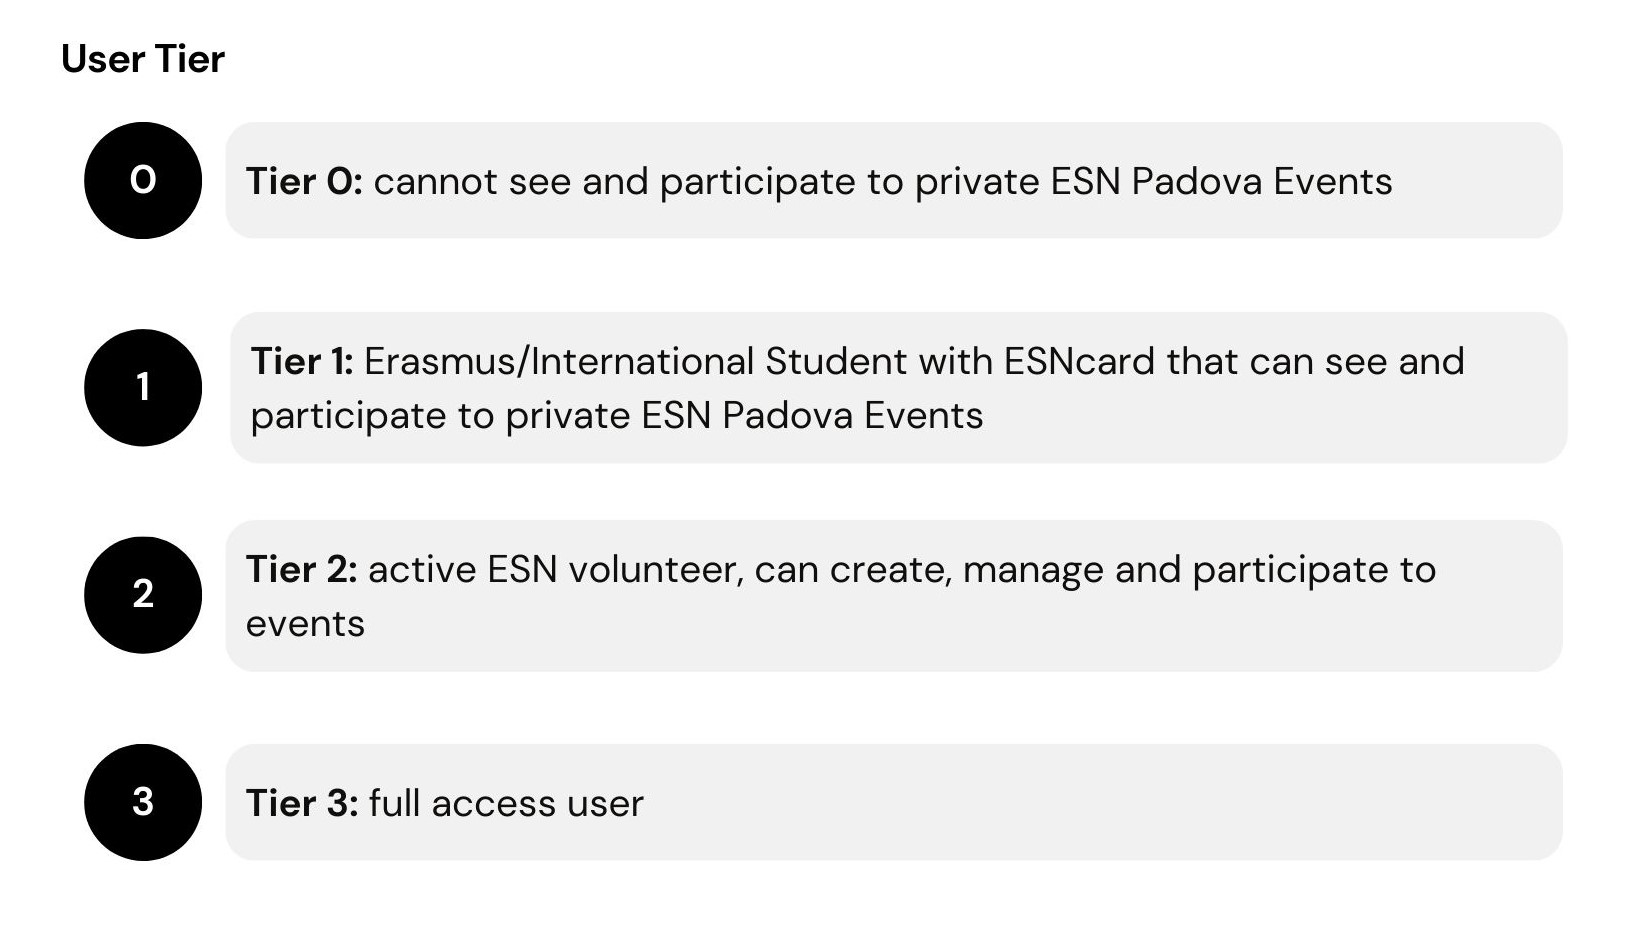
\includegraphics[width=0.5\textwidth]{images/tiers.jpg}
    \caption{Users tiers.}
    \label{fig:users_tiers}
\end{figure}